%%
%% Author: adriankunz
%% 2018-12-28
%%

% =============== Preamble ===============

% --------------- Definitions ---------------
\newcommand{\paperTitle}[0]{Valhalla}
\newcommand{\paperSubtitle}[0]{Seminar Java Features von Morgen, Sommersemester 2020}
\newcommand{\paperDate}[0]{\today}
\newcommand{\paperKeywords}[0]{Valhalla, Seminar, OpenJDK, Java}
\newcommand{\paperAuthor}[0]{Adrian Kunz}

% --------------- Document Setup ---------------
\documentclass[a4paper,12pt]{article}
\usepackage[left=2.5cm,right=2.5cm,top=2.5cm,bottom=2cm]{geometry}
\usepackage{setspace}
\onehalfspacing

\title{\paperTitle}
\author{\paperAuthor}
\date{\paperDate}

% --------------- Packages ---------------
\usepackage[ngerman]{babel}
\usepackage[T1]{fontenc}
\usepackage[utf8]{inputenc}
\usepackage{url}

% Minted
\usepackage{minted}
\usemintedstyle{vs}
\setminted{frame=single,tabsize=2,linenos}

\newmintinline[code]{java}{}
\newmintinline[plain]{text}{breaklines}

\setminted[java]{autogobble}

% Hyperref
\usepackage{hyperref}
\hypersetup{
pdftitle={\paperTitle{}},
pdfauthor={\paperAuthor{}},
pdfsubject={\paperTitle{}},
pdfkeywords={\paperKeywords},
bookmarksnumbered=true,
bookmarksopen=true,
hidelinks,
}
\usepackage{hypcap}

% To Do Commands
\usepackage{xcolor}

\newcommand{\todo}[1]{\textcolor{red}{TODO: #1}}
\newcommand{\todom}[1]{\marginpar{\parbox{1.5cm}{\textcolor{red}{TODO:\\ #1}}}}

% list of abbreviations
\usepackage[nolist]{acronym}

\begin{acronym}[xxx]
    \acro{api}[API]{Application Programming Interface}
    \acro{cpu}[CPU]{Central Processing Unit}
    \acro{jep}[JEP]{Java Enhancement Proposal}
    \acro{jvm}[JVM]{Java Virtual Machine}
\end{acronym}

\acused{api}
\acused{cpu}

% Units
\usepackage[binary-units=true]{siunitx}
\DeclareSIUnit\Byte{Byte}

\usepackage{amsmath}
\usepackage{graphicx}

% =============== Document ===============

\begin{document}

    \maketitle

    \section{Einleitung}\label{sec:introduction}

Als im Jahre 1995 die Programmiersprache Java von Sun Microsystems vorgestellt wurde, war heutige Hardware noch weit entfernt.
Speicherzugriffe und arithmetische Operationen hatten einen vergleichbaren Zeitaufwand und 64-Bit Systeme waren nur bei Servern und nicht für Endanwender vertreten.
Inzwischen hat sich die Hardware weiterentwickelt, während das Speichermodell der Sprache weitgehend unverändert blieb.
Das Projekt \emph{Valhalla} hat die Aufgabe, Java in diesem Aspekt zu modernisieren.
Um das zugrundeliegende Probleme darzustellen, wird zunächst in Abschnitt~\ref{sec:memory-model} das derzeitige Speichermodell von Java erläutert und einige Grundbegriffe definiert.
In Abschnitt~\ref{sec:valhalla} folgt dann ein Überblick über das Projekt Valhalla.
Darin wird auf die Geschichte des Projekts sowie damit verbundene Neuerungen für Java eingangen.
Zuletzt gibt Abschnitt~\ref{sec:summary} eine Zusammenfassung und einen Ausblick.

    \section{Das Speichermodell von Java}\label{sec:memory-model}

Das Speichermodell von Java beruht in erster Instanz auf \emph{Werten}.
Einfache Werte sind Zahlen in verschiedenen Größen und die boolschen Werte \code{true} und \code{false}.
Werte können in Variablen gespeichert werden und in Objekten verkapselt werden.
Objekte selber sind keine Werte, da sie nicht direkt in Variablen gespeichert werden können.
Einzig ist es möglich \emph{Referenzen} zu Objekten zu speichern.
Dabei handelt es sich um Verweise, die auf den eigentlichen Speicherort der Objektdaten zeigen.
Letzterer wird von der Java-Laufzeitumgebung verwaltet und ist nicht durch den Programmierer einsehbar.

% Indirektion
Um auf einen Wert in einem Objekt zuzugreifen, dessen Referenz in einer Variable gespeichert ist, muss diese zunächst \emph{dereferenziert} werden.
Dazu wird der Inhalt des Speichers an der Stelle geladen, auf die die Referenz zeigt.
Dies wird als \emph{Indirektion} bezeichnet, da der gesuchte Wert nicht direkt vorhanden ist.
Wenn Referenzen in einem Objekt gespeichert werden, benötigt ein Zugriff auf einen Wert in einem geschachtelten Objekt zwei Indirektionsschritte.
Es müssen folglich Daten von drei verschiedenen Orten im Speicher gelesen werden.

% Speicherebenen, Lokalität
Moderne Hardware organisiert den Speicher in verschiedene Ebenen.
\acp{cpu} haben neben den Registern, in denen die eigentliche Datenverarbeitung stattfindet, mehrere Cache-Ebenen, wo Daten aus dem Hauptspeicher zwischengelagert werden.
Während der Speicherplatz von Register über Cache zum Hauptspeicher mit jedem Schritt circa um den Faktor 1000 steigt, erhöhen sich auch die Zugriffszeiten in ähnlicher Größenordnung.
Gleichzeitig werden Daten stets in Blöcken von Hauptspeicher zum Cache kopiert, den sogenannten \emph{Cache-Zeilen}.
Folglich muss bei dreifachem Zugriff auf Daten, die nicht im gleichen Block im Arbeitsspeicher liegen, dreifach auf diesen zugegriffen werden.
Wenn stattdessen die Daten nah beieinander liegen, muss dies nur einmal geschehen -- dies wird als \emph{Lokalität} bezeichnet.

% Speicherverbrauch
Werte und Objekte haben eine feste Größe und damit einen Speicherverbrauch.
Zahlen vom Typ \code{int} sind beispielsweise 32 Bit und damit 4 Byte groß.
Referenzen haben eine feste Größe von 8 Byte auf einer 64-bit \ac{jvm}.
Der Speicherverbrauch eines Objekts berechnet sich aus der Summe der Größe der enthaltenen Werte plus einen Objekt-Header mit einer festen Größe von 16 Byte\footnote{Mit dem \ac{jvm}-Flag \code{-XX:+UseCompressedOops} könnte dies auf 12 Byte reduziert werden, allerdings kommen dann 4 Byte Padding hinzu, da die Größe von Objekten im Heap ein Vielfaches von 8 Byte sein muss~\cite{compressed-oops}.}.
Arrays, eine spezielle Art von Objekten mit einer variablen Anzahl von Elementen, berechnen ihren Speicherverbrauch aus einem 24 Byte großen Header plus die Summe des Speicherverbrauchs der Werte, die die Elemente bilden.
~\cite{compressed-oops}

% Beispiel
Es soll nun ein Beispiel betrachtet werden, um das Speichermodell von Java näher zu erläutern und die Probleme zu zeigen, die dadurch entstehen.
Modelliert werden einige ganzzahlige Punkte, die im zweidimensionalen Raum liegen und einen Pfad bilden sollen.
Die Punkte sind als Objekte mit zwei \code{int}-Feldern implementiert, der Pfad als Array von Punkten.
Es werden drei Punkte erstellt und in einem Array abgelegt, welches in einer Variable gespeichert wird.
Abbildung~\ref{fig:memory-usage} stellt diese Situation auf der linken Seite dar.

\begin{figure}[htp]
    \centering
    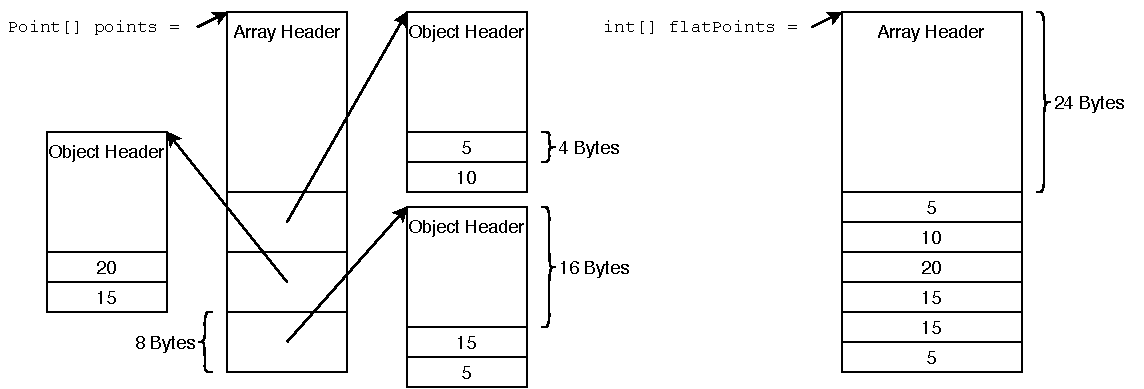
\includegraphics[width=\textwidth]{img/memory-usage.pdf}
    \vspace{-3ex}
    \caption{Vergleich des Speicherlayouts eines Arrays von Punkten (links) und von Zahlen (rechts)}
    \label{fig:memory-usage}
\end{figure}

Hier ist die doppelte Indirektion von der Variable bis zu einem der Punkte durch Verfolgen der Pfeile zu erkennen.
Um anhand der Variable auf einen Koordinate zuzugreifen, werden im schlechtesten Fall zwei Zugriffe auf den Hauptspeicher benötigt, da die Objekte an beliebigen Stellen darin liegen können.
Ebenfalls zu beachten ist der Speicherverbrauch, der sich wie folgt berechnet:

\begin{equation}
    \begin{split}
    \textit{Speicherverbrauch} & = \textit{Array-Header} + 3 \cdot (\textit{Referenz} + \textit{Objekt-Header} + 2 \cdot \textit{int}) \\
    & = \SI{24}{\Byte} + 3 \cdot (\SI{8}{\Byte} + \SI{16}{\Byte} + 2 \cdot \SI{4}{\Byte}) \\
    & = \SI{120}{\Byte}\label{eq:memory-usage-current} \\
    \end{split}
\end{equation}

Eine alternative Implementierung dieses Scenarios kann erfolgen, indem ein Array von \code{int-Werten} verwendet wird.
Dies wird auf der rechten Seite von Abbildung~\ref{fig:memory-usage} dargestellt.
Es fällt auf, dass ohne die zusätzlichen Objekte nicht dur die doppelte Indirektion, sondern auch die Objekt-Header entfallen.
Dadurch ergibt sich ein deutliche kleinerer Speicherverbrauch:

\begin{equation}
    \begin{split}
        \textit{Speicherverbrauch} & = \textit{Array-Header} + 6 * \textit{int} \\
        & = \SI{24}{\Byte} + 6 \cdot \SI{4}{\Byte} \\
        & = \SI{48}{\Byte}\label{eq:memory-usage-flat}
    \end{split}
\end{equation}

Folglich konnten $\SI{72}{\Byte}$ eingespart werden.
Der Effekt wird verstärkt, wenn das Array mehr Elemente enthält.
Zu beachten ist auch, dass die gesamten Daten des Arrays mit einer Größe von $\SI{48}{\Byte}$ in eine Cache-Zeile passen, wenn bei deren Größe von $\SI{64}{\Byte}$ ausgangen wird.

Ein Nachteil dieser Datenmodellierung ist, dass nun der Zugriff auf einzelne Koordinaten erschwert wird.
Statt \code{points[1].y} muss nun \code{flatPoints[3]} verwendet werden, um die y-Koordinate des zweiten Punkts im Array zu erhalten.
Das erschwert den Programmieraufwand und ist fehleranfälliger.
Weiterhin ist es nicht mehr direkt möglich, einen ganzen Punkt aus dem Array zur Weiterverarbeitung zu entnehmen.
Eine optimale Lösung wäre ein Kompromiss zwischen beiden Ansätzen, sodass beim Programmieren ein \code{Point[]} verwendet werden kann, während zur Laufzeit das Speicherlayout wie auf der rechten Seite von Abbildung~\ref{fig:memory-usage} aussieht.

% TODO woanders
%Neben Punkten lassen sich mit Value Types eine Vielzahl von neuen Datentypen definieren, die breite Anwendung finden können.
%Dazu gehören im Bereich der numerischen Datenverarbeitung komplexe, vorzeichenlose und Dezimalzahlen, Binärzahlen größer als 64 bit und Vektoren, die auf modernen \acp{cpu} effizient verarbeitet werden können.
%Auch algebraische Datentypen wie \code{Optional}, \code{Either}, \code{Unit} und Tupel sind wichtige Einsatzmöglichkeiten.
%Letztere benötigen jedoch besondere Sprachunterstützung, die noch nicht Teil des Projekts ist.

    \section{Projekt Valhalla}\label{sec:valhalla}

Das OpenJDK-Projekt \emph{Valhalla}~\cite{openjdk-valhalla} besteht aus drei wesentlichen Neuerungen, die in folgenden \acp{jep} definiert sind:

\begin{itemize}
    \itemsep0em
    \item \ac{jep} 169: Value Objects~\cite{jep-169}
    \item \ac{jep} 193: Variable Handles~\cite{jep-193}
    \item \ac{jep} 218: Generics over Primitive Types~\cite{jep-218}
\end{itemize}

Grundlage für die Änderungen des Projekts stellen die \emph{Value Objects} dar.
Deren Ziel ist es, die \ac{jvm} um Unterstützung für neue benutzerdefinierbare Typen zu erweitern, die \emph{Value Types}.
Diese haben im Vergleich zu bestehenden Klassen keine Referenzsemantik, sondern verhalten sich wie primitive Datentypen.
\ac{jep} 169 selber beschäftigt sich nur mit einer kleinen Erweiterung der \ac{jvm} in diese Richtung.
Unterabschnitt~\ref{subsec:value-types} betrachtet die Value Types als Gesamtkonzept.

Die \emph{Variable Handles} bezeichnen einen Teil der Java-Standardbibliothek, die präziseren Zugriff auf Felder von Objekten und Array-Elementen ermöglichen.
Die Implementierung der \ac{api} erfolgte bereits in Java 9 und wird daher nicht näher in dieser Arbeit betrachtet.

Die Erweiterung von generischen Typen um Unterstützung für primitive Typen ist der größte Teil des Projekts.
Sie verlangt weitreichende Änderungen, die sowohl die Sprache als auch die \ac{jvm} betreffen.
In Unterabschnitt~\ref{subsec:primitive-generics} erfolgt eine Vertiefung in dieses Thema.

\subsection{Value Types}\label{subsec:value-types}

Seit der ersten Version von Java wird der Ansatz verfolgt, dass alles außer primitiven Werten ein Objekt ist.
Das unterscheided Java von Programmiersprachen wie C oder C++, wo primitive Werte sowie Klassen und Structs zunächst nur einfache Werte sind und erst durch Pointer eine Referenzsemantik erhalten.

In Java sind hingegen alle Variablen und Parameter vom Typ einer Klasse implizit Pointer, die automatisch von der \ac{jvm} verwaltet werden.
Dies vereinfacht das Programmiermodell und ist weniger fehleranfällig, besonders durch den Garbage Collector.
Es führt jedoch auch dazu, dass alle Zugriffe auf Daten in diesen Objekten über Indirektion erfolgen.
Dies verringert die Lokalität der Daten und resultiert auf heutiger Hardware in deutlich langsamerer Performance.
Weiterhin erzeugen Referenzen einen deutlichen höheren Speicherverbrauch, wie ein Beispiel in Abschnitt~\ref{subsubsec:memory-example} zeigen wird.
Zuletzt sorgt die Allokation und Freigabe des Speichers, besonders bei einer Vielzahl kleiner Objekte, für einen Verwaltungsaufwand seitens des Allocators und Garbage Collectors.

Aufgrund dieser Performance-\ und Speicherbedenken suchen viele Java-Entwickler nach Möglichkeiten, Klassen und Objekte zu umgehen.
Meist entsteht dabei Code, der händische Optimierungen auf Kosten von Lesbarkeit, Abstraktion und Fehlersicherheit enthält.
Value Types sollen dies vermeiden.

\subsubsection{Unterschiede zu Referenztypen}

Es soll nun betrachtet werden, was Value Types von regulären Referenztypen unterscheided.
Größter Unterschied ist, dass nun keine Pointer mehr verwendet werden, ohne die sich einige grundlegende Konzepte ändern.
So besitzen Werte keine Identität mehr, die verglichen werden könnte, und damit auch keinen Identitäts-Hashcode.
Die Veränderung der Felder von Werten ist entweder nicht erlaubt oder wirkt sich nur auf lokale Instanzen in Variablen und Parametern aus, da Value Types wie primitive Werte bei jeder Zuweisung kopiert werden.
Durch die Kopier-Semantik können Werte nicht mehr als Monitor für die Synchronisierung dienen und auch die \code{clone}-Operation ist nicht mehr sinnvoll.
Ebenso ist der Finalizer nun überflüssig, da die Werte nicht mehr vom Garbage Collector verarbeitet werden.
Auch \code{null} ist kein gültiger Wert mehr, allerdings wäre eine Alternative möglich, die den Speicher für den Wert auf null setzt.
Zuletzt kann nicht von Value Types geerbt werden, da im Voraus bekannt sein muss, wie viel Speicherplatz reserviert werden muss, was mit Vererbung nicht statisch entschieden werden kann.

\subsubsection{Value-basierte Klassen}

Seit Java 8 definiert die Sprache bereits ein Konzept, das den Value Types ähnelt: die Value-basierten Klassen~\cite{value-based-classes}.
Dabei handelt es sich um eine Konvention, die von einigen Klassen der Standardbibliothek eingehalten wird und auch für Bibliotheksautoren und andere Endbenutzer der Sprache verfügbar ist.
Wesentlich bei Value-basierten Klassen ist der Einsatz von Feldern, die \code{final} sind, wodurch Instanzen dieser Klassen unveränderbar sind.
Weiterhin dürfen diese Klassen keinen öffentlich zugänglichen Konstruktor besitzen, sondern müssen stets über eine Factory-Methode instanziiert werden.
Dadurch müssen keine Garantien über die Identität erstellter Objekte gemacht werden.
Die Factory-Methode kann beispielsweise ihre Rückgabewerte in einem Cache speichern.
Aufgrund der fehlenden Identität ist es nicht sinnvoll, Identitätsvergleiche mit \code{==} durchzuführen.
Folglich müssen stets \code{equals} und \code{hashCode} implementiert werden.
Identitäts-basierte Operationen und Synchronisierung auf Value-basierten Klassen sind zwar derzeit nicht verboten, da es sich um eine Konvention handelt, können aber zu unerwarteten Ergebnissen führen.
Somit erfüllen Value-basierte Klassen fast alle zuvor genannten Punkte, durch die sich Value Types von Referenztypen unterscheiden.
Ausnahmen sind \code{null} als möglicher Wert sowie die erlaubte Vererbung.
Beides ist jedoch bei derzeitigen Beispielen für Value-basierte Klassen wie \code{Integer} und \code{Optional} ohnehin nicht üblich.

\subsubsection{Inline-Klassen}

Mit dem Projekt Valhalla soll die Konvention der Value-basierten Klassen nun Sprach- und \ac{jvm}-Unterstützung erhalten.
Diese trägt die Bezeichnung \emph{Inline-Klassen}~\cite{object-model}, die sich aus dem Schlüsselwort \code{inline} ableitet, das für die Deklaration von Value Types eingesetzt wird.
Listing~\ref{inline-class-example} zeigt, wie eine Inline-Klasse aussehen kann.
Dabei ist zu beachten, dass sich der Code nur durch das Schlüsselwort \code{inline} von einer regulären Klasse unterscheidet.
Nach dem Motto ``Codes like a class, works like an int''~\cite{object-model} sollen die syntaktischen Änderungen bewusst klein sein.

\begin{listing}
    \begin{minted}{java}
        inline class Point {
            private int x, y;

            public Point(int x, int y) { this.x = x; this.y = y; }

            public int x() { return x; }
            public int y() { return y; }
        }
    \end{minted}
    \vspace{-3ex}
    \caption{Beispiel für eine Inline-Klasse (angepasst aus~\cite{object-model})}
    \label{inline-class-example}
\end{listing}

% Primitive untergeordnet
Mit der Einführung von Inline-Klassen wird die Unterscheidung zwischen primitiven und Referenz-Typen abgeschafft.
Nun wird zwischen Inline- und Referenz-Typen unterschieden;
die primitiven Typen werden den Inline-Typen untergeordnet.
% T.default
Weiterhin kann nun für alle Typen ein Default-Wert definiert werden, der mit \code{T.default} bezeichnet wird.
Für primitive Typen bleibt dieser \code{0} oder \code{false}, während Referenztypen \code{null} beibehalten.
Inline-Typen definieren ihren Default-Wert als eine Instanz, bei der alle Felder mit dem jeweiligen Default-Wert belegt sind.

% Marker interfaces
Unter Umständen kann es nützlich sein, zur Laufzeit zu ermitteln, ob es sich bei einem Wert um eine Referenz oder einen Inline-Wert handelt.
Dafür werden neue Interfaces eingeführt, von denen automatisch und implizit alle Klassen erben:
\code{IdentityObject} für Referenzen und \code{InlineObject} für Inline-Klassen.
So kann entschieden werden, ob Identitätsoperationen wie \code{==} oder Synchronisierung sinnvoll sind.
% Interfaces + Klassenvererbung
Inline-Klassen dürfen auch reguläre Interfaces implementieren.
Ebenfalls können sie von Klassen ohne \code{inline} erben, solange diese nicht den Anforderungen an Inline-Klassen widersprechen.
Nicht erlaubt wären beispielsweise Superklassen mit nicht-finalen Feldern oder Methoden, die \code{synchronized} sind.
Ein Beispiel für eine Klasse, welche die Anforderungen erfüllt, ist \code{Object}, von der weiterhin alle Klassen erben.

% Boxing
Mit der Unterordnung von primitiven Typen werden auch diese ohne Boxing von \code{Object} erben.
Boxing wird dann zu einer Operation, die von der \ac{jvm} intern durchgeführt wird und nicht mehr nur durch den Compiler bereitgestellter syntaktischer Zucker ist.
% Arrays
Das hat zur Folge, dass Array-Typen anders voneinander erben.
Insbesondere kann nun ein \code{int[]} direkt in ein \code{Integer[]} oder ein \code{Object[]} umgewandelt werden.
Ein ähnliches Verhalten zeigen die benutzerdefinierten Inline-Klassen.
% Referenz-Wrapper T.ref
Anders als bei primitiven Typen gibt es jedoch dafür keine explizit definierten Referenz-Wrapper.
Stattdessen soll neue Syntax hinzugefügt werden, mit der Referenz-Wrapper für Inline-Klassen benannt werden können.
Diese nimmt die Form \code{T.ref} an, wobei \code{T} eine Inline-Klasse bezeichnet.
Im Gegensatz dazu steht die Form \code{T.val}, die explizit den Inline-Typ benennt.
Diese Formen sollen mit den bestehenden Namen für primitive und Wrapper-Typen kompatibel sein -- \code{int.ref} bezeichnet dann den selben Typ wie \code{Integer} und \code{Integer.val} entspricht \code{int}.

\subsubsection{Beispiel zum Speicherverbrauch}\label{subsubsec:memory-example}

Um das Speicherproblem näher zu erläutern, soll nun ein Beispiel betrachtet werden.
Es sollen einige ganzzahlige Punkte im zweidimensionalen Raum gespeichert werden, die einen Pfad bilden.
Die Punkte sind als Objekte mit zwei \code{int}-Feldern modelliert, der Pfad als Array von Punkten.
Bei einer Pfadlänge von drei berechnet sich der Speicherverbrauch wie folgt:

\begin{equation}
    \SI{24}{\Byte} + 3 \cdot \SI{8}{\Byte} + 3 \cdot (\SI{16}{\Byte} + 2 \cdot \SI{4}{\Byte}) = \SI{120}{\Byte}\label{eq:memory-usage-current}
\end{equation}

Die Größe eines Array-Headers beträgt $\SI{24}{\Byte}$~\cite{compressed-oops}.
Ein Objekt, das zwei \code{int}-Werte beeinhaltet, benötigt auf einer 64-bit \ac{jvm} $\SI{8}{\Byte}$ für die Referenz selber, $\SI{16}{\Byte}$\footnote{Mit dem \ac{jvm}-Flag \code{-XX:+UseCompressedOops} könnte dies auf $\SI{12}{\Byte}$ reduziert werden, allerdings kommen dann $\SI{4}{\Byte}$ Padding hinzu, da die Größe von Objekten im Heap ein Vielfaches von $\SI{8}{\Byte}$ sein muss~\cite{compressed-oops}.} für den Objekt-Header und je $\SI{4}{\Byte}$ für die beiden \code{int}-Werte~\cite{compressed-oops}.
Mit drei Objekten ergibt sich also insgesamt ein Speicherverbrauch von $\SI{120}{\Byte}$.

Das gleiche Beispiel soll nun mit Value Types realisiert werden.
Dabei entfallen die Objekt-Header und Referenzen vollständig.
Der neue Speicherverbrauch berechnet sich also wie folgt:

\begin{equation}
    \SI{24}{\Byte} + 3 \cdot 2 \cdot \SI{4}{\Byte} = \SI{48}{\Byte}\label{eq:memory-usage-inline}
\end{equation}

Folglich konnten $\SI{72}{\Byte}$ eingespart werden.
Der Effekt wird verstärkt, wenn das Array mehr Elemente enthält.
Zu beachten ist auch, dass die gesamten Daten des Arrays mit einer Größe von $\SI{48}{\Byte}$ in eine Cache-Zeile passen, wenn bei deren Größe von $\SI{64}{\Byte}$ ausgangen wird.

In Abbildung~\ref{fig:memory-usage} erfolgt eine grafische Darstellung des verringerten Speicherverbrauchs.
Sie zeigt links das Speicherlayout in heutigen \acp{jvm} und rechts das Speicherlayout, wenn Value Types für die Punkte verwendet werden.

\begin{figure}
    \centering
    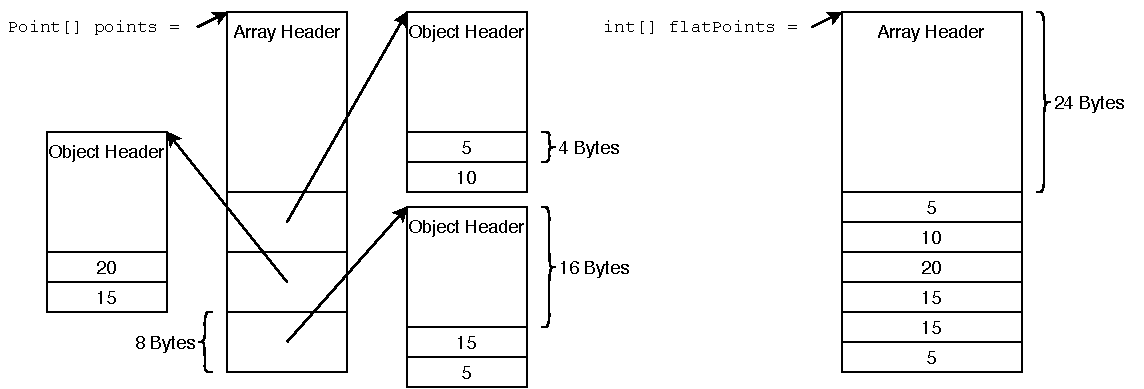
\includegraphics[width=\textwidth]{img/memory-usage.pdf}
    \vspace{-3ex}
    \caption{Vergleich des Speicherlayouts eines Arrays von Punkten heute (links) und mit Value Types (rechts)}
    \label{fig:memory-usage}
\end{figure}

Neben Punkten lassen sich mit Value Types eine Vielzahl von neuen Datentypen definieren, die breite Anwendung finden können.
Dazu gehören im Bereich der numerischen Datenverarbeitung komplexe, vorzeichenlose und Dezimalzahlen, Binärzahlen größer als 64 bit und Vektoren, die auf modernen \acp{cpu} effizient verarbeitet werden können.
Auch algebraische Datentypen wie \code{Optional}, \code{Either}, \code{Unit} und Tupel sind wichtige Einsatzmöglichkeiten.
Letztere benötigen jedoch besondere Sprachunterstützung, die noch nicht Teil des Projekts ist.

\subsection{Primitive und generische Typen}\label{subsec:primitive-generics}

Generische Typen sind ein Feature, das bereits in Java 5 eingeführt wurde.
Sie ermöglichen es, Klassen und Methoden zu definieren, die über verwendete Typen abstrahieren.
Dabei kommen Typparameter als Platzhalter zum Einsatz.
So kann beispielsweise eine \code{Map}-Klasse erstellt werden, bei der Schlüssel und Werte beliebig, aber fest typisiert sind.
Bei der Verwendung der Klasse werden die Typen festgelegt: \code{Map<String, Integer>}.
Dadurch können typsichere Datenstrukturen definiert werden.

\subsubsection{Erasure}

Die Implementierung von generischen Typen erfolgte durch die sogenannte \emph{Erasure}.
Beim Generieren von Bytecode ersetzt der Java-Compiler sämtliche Vorkommen von generischen Typparametern durch \code{Object}\footnote{Falls durch die Form \code{<T extends Bound>} ein Bound angegeben wird, wird der Typparameter durch diesen statt \code{Object} ersetzt.}.
Generische Typen konnten so implementiert werden, ohne Änderungen an der \ac{jvm} vornehmen zu müssen.
Erasure steht im Kontrast zur Spezialisierung, bei der Typparameter wie bei einer Vorlage durch die konkreten Typen ersetzt werden, als wären sie direkt in der Klasse oder Methode verwendet worden.
Dieser Ansatz wird beispielsweise von C++ benutzt.
Er hat den Vorteil, dass typspezifische Optimierungen durchgeführt werden können und Spezialisierungen eigene Methoden und sonstige Funktionalität bereitstellen können.
Nachteil ist jedoch die Duplizierung von Code, wodurch Binärdateien größer werden.
Zudem sind sogenannte \emph{Wildcard-Typen} mit vollständiger Spezialisierung nicht möglich.
Ein Wildcard-Typ wie \code{List<?>} bildet in Java einen gemeinsamen Supertyp von allen Typen \code{List<T>} mit beliebigem Typ \code{T}.

% Migration mit Erasure
Erasure ermöglichte ferner den Entwicklern, schrittweise auf generische Typen umsteigen.
Die Benutzung von \code{Map} war weiterhin ohne Angabe der Schlüssel- und Wert-Typen erlaubt -- dies wird als Raw Type bezeichnet und verhält sich ähnlich wie \code{Map<Object, Object>}.
Die Wahrung der Kompatibilität war ein besonderes Ziel bei der Entwicklung der generischen Typen.
Es sollte vermieden werden, dass Entwickler sämtlichen Code neu kompilieren müssen.

% Keine generischen Typen mit Primitives
Eine Limitierung der Erasure ist, dass primitive Typen nicht als Typparameter verwendet werden können.
So erzeugt der Compiler derzeit einen Error, wenn der Typ \code{List<int>} verwendet wird.
Das liegt daran, dass der Typ \code{int} derzeit nicht kompatibel mit \code{Object} ist.
Nur durch Boxing kann die Umwandlung \code{int <-> Integer <-> Object} geschehen.
Dies kann aber in generischen Klassen nicht sichergestellt werden, solange der konkrete Typ nicht bekannt ist.
Folglich muss statt \code{List<int>} eine \code{List<Integer>} verwendet werden.
Zur Laufzeit kann dies jedoch aufgrund des Boxings die Performance beeinträchtigen:
Sowohl das Boxing (Anlegen von \code{Integer}-Objekten) als auch das Unboxing (Extrahieren des \code{int}-Werts) benötigt Zeit, besonders aufgrund des Allokations- und Garbage-Collector-Overheads sowie der zusätzlichen Indirektion.
Der erhöhte Speicherverbrauch, der bereits im vorherigen Unterabschnitt~\ref{subsec:value-types} gezeigt wurde, ist auch hier in ähnlichem Umfang vorhanden.

\subsubsection{Händische Spezialisierung}

Aufgrund von Bedenken zu Performance und Speicherverbrauch sind in Java-Bibliotheken häufig händische Spezialisierungen vertreten.
Beispiele dafür sind selbst in der Standardbibliothek zu finden.
So gibt es seit Java 8 die Klassen \code{OptionalInt} und \code{IntStream} sowie Äquivalente für \code{long} und \code{double}, die als performanter und speichersparender Ersatz für \code{Optional<T>} und \code{Stream<T>} dienen und untereinander nicht kompatibel sind~\cite{java-8-docs}.
Das Problem wird verstärkt, wenn die zu spezialisierende Klasse mehr als einen Typparameter hat.
Im Package \code{java.util.function} ist eine Reihe von Spezialisierungen für Interfaces vorhanden, die je eine Methode mit null, einem oder zwei Parametern bereitstellen, deren Typen generisch sind.
Mehrere Klassen variieren ebenfalls im Rückgabetyp der Methode.
Händische Spezialisierungen können zwar für verbesserte Performance sorgen, besonders wenn typspezifische Optimierungen vorgenommen werden, erzeugen aber einen erhöhten Wartungsaufwand und sind fehleranfälliger.

% Einfluss von Value Types
In bisherigen Java-Versionen ist das Problem nur auf die acht primitiven Typen beschränkt.
Werden diese acht auf die drei häufigsten -- \code{int}, \code{long} und \code{double} -- reduziert, kann die Anzahl der händischen Spezialisierungen eingeschränkt werden.
Dies ist jedoch nicht mehr möglich, wenn mit Value Types eine unendliche Zahl neuer Typen hinzukommen, die sich ähnlich wie primitive verhalten sollen.
Es wäre nicht sinnvoll, den Speicherverbrauch von Arrays zu verringern, wenn das nicht auch mit Listen möglich ist, da diese in den meisten Fällen die bessere Wahl sind.
Folglich ist es naheliegend, dass die Änderung von generischen Typen zusammen mit den neuen Value Types eingeführt wird.

\subsubsection{Spezialisierung durch den Compiler}

Ein Ansatz, der das Wartungsproblem der händischen Spezialisierung vermeidet, ist Spezialisierung durch den Compiler.
Dabei erzeugt der Compiler aus einer Quellcode-Datei mehrere Bytecode-Dateien für eine vorgegebene Menge von Typen.
Dies kommt beispielsweise in der \ac{jvm}-Sprache \emph{Scala} zum Einsatz, in der Spezialisierungen mit einer Annotation an einem Typparameter festgelegt werden können~\cite{scala-specialized}.
Das verringert zwar den Programmieraufwand, sorgt aber dennoch für größere Artefakte aufgrund des duplizierten Bytecodes.
Zudem sind die entstehenden Klassen aus Sicht der \ac{jvm} und anderen Java-ähnlichen Sprachen nicht verwandt, wodurch spezielle Interfaces verwendet werden müssen, wenn beispielsweise ein Wildcard-Typ gebraucht wird.
Weiterhin wird Reflection erschwert, was in Scala durch eine eigene Reflection-Bibliothek umgangen wird.
Eine solche Vorgehensweise ist in zukünftigen Java-Versionen aufgrund von Kompatibilitätsbedenken also nicht erstrebenswert.

\subsubsection{Spezialisierung zur Laufzeit}

Eine kompatible und nachhaltige Implementierung von generischer Spezialisierung erfordert folglich Unterstützung durch die Laufzeitumgebung.
Bereits im Jahr 2014 wurde an einem ersten Prototyp gearbeitet, der Teile der Spezialisierung auf die Laufzeit auslagert~\cite{specialization}.
Der Java-Compiler erzeugt dann nur eine Bytecode-Datei pro Klasse, von der ausgehend Spezialisierungen zur Laufzeit erzeugt werden, wenn sie benötigt werden.
Dafür mussten Metadaten im Bytecode-Format hinzugefügt werden, die Angaben über verwendete Typparameter machen, die bei der reinen Erasure zuvor nicht notwendig waren.
Ein wichtiges Ziel war es, die Spezialisierung zur Laufzeit so einfach wie möglich zu halten und zusätzliche Verifikation oder komplexe Übersetzungsverfahren zu vermeiden.
Das sollte die Implementierung vereinfachen und Ladezeiten gering halten, setzte aber bedachte Änderung des Bytecode-Formats voraus.

\subsubsection{Syntaktische Neuerungen}

% any
Zum aktuellen Zeitpunkt ist noch keine endgültige Syntax für generischen Typen mit Spezialisierung festgelegt.
Es ist naheliegend, dass aus Kompatibilitätsgründen die bestehende Syntax für Typparameter die Semantik der Erasure beibehalten wird und Spezialisierung explizit aktiviert werden muss.
Dafür wurde in der Literatur zu Valhalla vorläufig das Schlüsselwort \code{any} verwendet: \code{class Box<any T>}.

% Layers
Eine weitere vorgeschlagene syntaktische Neuerung sind die \emph{Layers}, welche es ermöglichen, in bestimmten Spezialisierungen neue Methoden hinzuzufügen.
Sie sind aus dem Problem entstanden, dass die meisten bestehenden generischen Klassen unter der Annahme implementiert wurden, dass sie nur mit Referenztypen verwendet werden.
So kann beispielsweise die Methode \code{V get(K key)} der Klasse \code{Map<K, V>} \code{null} zurückgeben, wenn der Schlüssel nicht vorhanden ist.
Dies ist jedoch nicht möglich, wenn \code{V=int} ist.
Mithilfe von Layers kann nun festgelegt werden, dass es die \code{get}-Methode nur dann geben soll, wenn \code{V} ein Referenztyp ist.
Andernfalls könnte eine neue Methode \code{getOrDefault} hinzugefügt werden.
Listing~\ref{lst:map-layer} zeigt, wie dies im Code definiert werden könnte.
Das Schlüsselwort \code{layer} gibt hier die Methoden an, die nur in der Spezialisierung für Referenztypen \code{V} existieren sollen.
Ähnliche Syntax könnte eingesetzt werden, um gänzlich neue Methoden wie \code{List<int>.sum()} hinzuzufügen.

\begin{listing}
    \begin{minted}{java}
        interface Map<any K, any V> {
            V getOrDefault(K key, V defaultValue);

            layer<ref V> {
                V get(K key);

                default V getOrDefault(K key, V defaultValue) {
                    return containsKey(key) ? get(key) : defaultValue;
                }
            }
        }
    \end{minted}
    \vspace{-3ex}
    \caption{Beispieldefinition des Map-Interfaces mit Layers (aus~\cite{specialization}).}
    \label{lst:map-layer}
\end{listing}

% Weitere Probleme
Layer sind eine Lösung für eines von vielen konzeptionellen und implementierungsbezogenen Problemen mit der Spezialisierung.
Weitere Hindernisse bei Wildcard-Typen, Arrays, Reflection und anderen Bereichen der Sprache sind in~\cite{jep-218} und~\cite{specialization} näher erläutert.

    \section{Zusammenfassung}\label{sec:summary}

% Zusammenfassung
Aus dem Wunsch, die Sprache Java für heutige Hardware zu modernisieren, hat sich mit Valhalla ein großes und aufwendiges Projekt entwickelt.
Die Value Types erfordern zwar nur kleine syntaktische Änderungen, dafür jedoch weitreichende Änderungen der \ac{jvm}.
Mehr sprachliche Neuerungen und Probleme entstehen jedoch durch die generische Spezialisierung, die nicht nur für primitive Datentypen interessant ist, sondern auch große Bedeutung für den Erfolg von Value Types hat.

Seit die Entwicklung des Projekts im Jahre 2014 begann, wurden viele Lösungansätze untersucht und in Form verschiedener Prototypen umgesetzt.
Da stets die Kompatibilität im Vordergrund stand, mussten die weitreichenden Änderungen genau abgewägt und analysiert werden.
Im Jahr 2020 ist mit den Inline-Klassen ein vielversprechendes Konzept vorhanden, das bei ersten Tests zwar gut funktionierte, aber noch nicht alle Versprechen erfüllen konnte.
Daher ist es naheliegend, dass die Entwicklung der Value Types noch weitere Zeit in Anspruch nehmen wird.

Auch auf dem Weg zur generischen Spezialisierung sind viele Prototypen entstanden, die zum Teil einfach umzusetzen waren, aber unterschiedlich viele Probleme und Bedenken mit sich führten.
Der neueste Ansatz der Spezialisierung zur Laufzeit verlangt zwar einen hohen Implementierungsaufwand seitens der \ac{jvm}-Autoren, bietet aber bessere Optimierungsmöglichkeiten als andere Ansätze.
% Ausblick
Insgesamt ist die Implementierung der generischen Spezialisierung stark von der Umsetzung der Value Types abhängig.
Da beide Features noch unvollständig umgesetzt sind, ist derzeit nicht absehbar, wann sie in einer Java-Version veröffentlich werden.


    \bibliographystyle{unsrtdin}
    \begingroup
    \linespread{0}\selectfont % condense the bibliography entries
    \bibliography{main}
    \endgroup

\end{document}
